% ============================================================
%  Área e Perímetro — Apostila Premium | PratiqueJá
%  Engine: XeLaTeX
% ============================================================
\documentclass[12pt]{article}
\usepackage{../../pratiqueja}
\usepackage{tikz}

\newcommand{\hlm}[1]{{\color{darkblue}#1}}

\setsubject{Área e Perímetro}

% Estilos TikZ reutilizáveis
\tikzset{
  figno/.style={draw=none, fill=none, black!60!white, font=\small\bfseries},
  figlines/.style={line width=1.8pt},
  figrect/.style={line width=1pt},
  sq/.style={figlines, draw=violet!80!black, fill=violet!12!white},
  ret/.style={figlines, draw=pink!70!black,  fill=pink!12!white},
  par/.style={figlines, draw=green!50!black,  fill=green!10!white},
  tri/.style={figlines, draw=violet!70!black, fill=violet!12!white},
  teq/.style={figlines, draw=blue!70!black,   fill=blue!12!white},
  trap/.style={figlines, draw=pink!70!black,  fill=pink!12!white},
  los/.style={figlines, draw=orange!70!black, fill=orange!12!white},
  circ/.style={figlines, draw=yellow!60!black,fill=yellow!10!white},
}

\begin{document}
\pagenumbering{arabic}
\setstretch{1.2}
\color{bodytext}

\heroheader{Área e Perímetro}%
           {Fórmulas das Principais Figuras Planas}%
           {Matemática · Básico}

\setlength{\columnsep}{18pt}
\setlength{\columnseprule}{0.5pt}
\def\columnseprulecolor{\color{exborder}}

\begin{multicols}{2}

%─────────────────────────────────────────────────────────────
\TW{Def}{badgepurple}{Definição}{Área e Perímetro}

\regra{A \textbf{área} de uma figura plana é a medida da superfície
que ela ocupa — imagine a figura coberta por quadradinhos de lado 1;
a quantidade de quadradinhos é a área. A unidade é sempre
\textbf{quadrática}: cm², m², km²…}

\regra{O \textbf{perímetro} de um polígono é a soma de todos os seus
lados — a medida total do contorno. A unidade é \textbf{linear}:
cm, m, km…}

\formula{$P = l_1 + l_2 + \cdots + l_n$}

%─────────────────────────────────────────────────────────────
\TW{Quad}{darkblue}{Quadrado}{Todos os lados iguais, ângulos retos}

\begin{center}\vspace{-4pt}
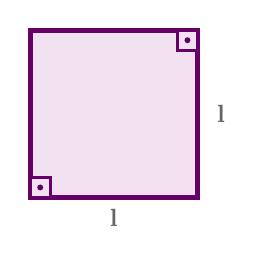
\begin{tikzpicture}[scale=0.85]
\draw[sq] (0,0) rectangle (2.5,2.5);
\node[figno] at (1.25,-0.3) {l};
\node[figno] at (2.85,1.25) {l};
\draw[sq,figrect] (0,0) rectangle (0.3,0.3);
\filldraw[violet!80!black] (0.15,0.15) circle (1pt);
\draw[sq,figrect] (2.5,2.5) rectangle (2.2,2.2);
\filldraw[violet!80!black] (2.35,2.35) circle (1pt);
\end{tikzpicture}
\vspace{-4pt}\end{center}

\regra{$A = l^2 \qquad P = 4\,l$}

\exemp{%
  Exemplo — $l = 5$\\
  $A = 5^2 = \hlm{25}$ \quad $P = 4 \cdot 5 = \hlm{20}$%
}

%─────────────────────────────────────────────────────────────
\TW{Ret}{darkblue}{Retângulo}{Lados opostos iguais, ângulos retos}

\begin{center}\vspace{-4pt}
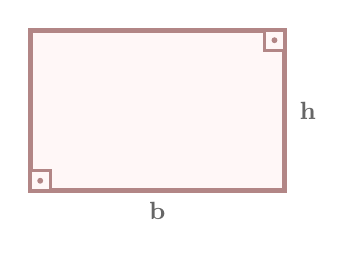
\begin{tikzpicture}[scale=0.85]
\draw[ret] (0,0) rectangle (3.8,2.4);
\node[figno] at (1.9,-0.3) {b};
\node[figno] at (4.15,1.2) {h};
\draw[ret,figrect] (0,0) rectangle (0.3,0.3);
\filldraw[pink!70!black] (0.15,0.15) circle (1pt);
\draw[ret,figrect] (3.8,2.4) rectangle (3.5,2.1);
\filldraw[pink!70!black] (3.65,2.25) circle (1pt);
\end{tikzpicture}
\vspace{-4pt}\end{center}

\regra{$A = b \cdot h \qquad P = 2\,(b + h)$}

\exemp{%
  Exemplo — $b = 4,\; h = 3$\\
  $A = 4 \cdot 3 = \hlm{12}$ \quad $P = 2 \cdot (4+3) = \hlm{14}$%
}

%─────────────────────────────────────────────────────────────
\TW{Par}{darkblue}{Paralelogramo}{Lados opostos paralelos e iguais}

\begin{center}\vspace{-4pt}
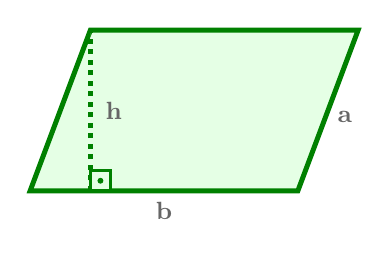
\begin{tikzpicture}[scale=0.85]
\draw[par] (0,0) -- (0.9,2.4) -- (4.9,2.4) -- (4,0) -- cycle;
\node[figno] at (2,-0.3) {b};
\node[figno] at (4.7,1.1) {a};
\node[figno] at (1.25,1.2) {h};
\draw[par,dotted] (0.9,0) -- (0.9,2.4);
\draw[par,figrect] (0.9,0) rectangle (1.2,0.3);
\filldraw[green!50!black] (1.05,0.15) circle (1pt);
\end{tikzpicture}
\vspace{-4pt}\end{center}

\regra{$A = b \cdot h \qquad P = 2\,(a + b)$\\[2pt]
{\small $b$ = base, $h$ = altura perpendicular, $a$ = lado oblíquo}}

\exemp{%
  Exemplo — $b = 5,\; h = 2,\; a = 4$\\
  $A = 5 \cdot 2 = \hlm{10}$ \quad $P = 2 \cdot (4+5) = \hlm{18}$%
}

%─────────────────────────────────────────────────────────────
\TW{Tri}{darkblue}{Triângulo}{Base e altura perpendicular}

\begin{center}\vspace{-4pt}
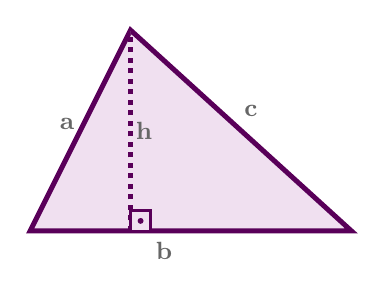
\begin{tikzpicture}[scale=0.85]
\draw[tri] (0,0) -- (4.8,0) -- (1.5,3) -- cycle;
\draw[tri,dotted] (1.5,0) -- (1.5,3);
\node[figno] at (1.7,1.5) {h};
\node[figno] at (0.55,1.6) {a};
\node[figno] at (3.3,1.8) {c};
\node[figno] at (2,-0.3) {b};
\draw[tri,figrect] (1.5,0) rectangle (1.8,0.3);
\filldraw[violet!70!black] (1.65,0.15) circle (1pt);
\end{tikzpicture}
\vspace{-4pt}\end{center}

\regra{$\displaystyle A = \frac{b \cdot h}{2} \qquad P = a + b + c$}

\exemp{%
  Exemplo — $b = 6,\; h = 3,\; a = 3,\; c = 5$\\
  $A = \dfrac{6 \cdot 3}{2} = \hlm{9}$ \quad $P = 3+6+5 = \hlm{14}$%
}

\nota{A \textbf{altura} é sempre perpendicular à base — pode cair
\emph{fora} do triângulo nos casos obtusângulos.}

%─────────────────────────────────────────────────────────────
\TW{Equi}{darkblue}{Triângulo Equilátero}{Três lados iguais, ângulos de 60°}

\begin{center}\vspace{-4pt}
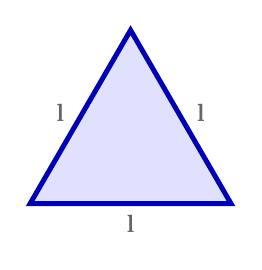
\begin{tikzpicture}[scale=0.85]
\draw[teq] (0,0) -- (3,0) -- (1.5,2.59) -- cycle;
\node[figno] at (1.5,-0.3) {l};
\node[figno] at (0.45,1.35) {l};
\node[figno] at (2.55,1.35) {l};
\end{tikzpicture}
\vspace{-4pt}\end{center}

\regra{$\displaystyle A = \frac{l^2\sqrt{3}}{4} \qquad P = 3\,l$}

\exemp{%
  Exemplo — $l = 4$\\
  $A = \dfrac{16\sqrt{3}}{4} = 4\sqrt{3} \approx \hlm{6{,}93}$\\[4pt]
  $P = 3 \cdot 4 = \hlm{12}$%
}

\nota{A altura do equilátero é $h = \dfrac{l\sqrt{3}}{2}$,
o que origina a fórmula da área.}

%─────────────────────────────────────────────────────────────
\TW{Trap}{darkblue}{Trapézio}{Um par de lados paralelos (bases)}

\begin{center}\vspace{-4pt}
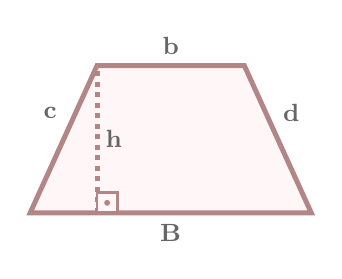
\begin{tikzpicture}[scale=0.85]
\draw[trap] (0,0) -- (1,2.2) -- (3.2,2.2) -- (4.2,0) -- cycle;
\node[figno] at (2.1,-0.3) {B};
\node[figno] at (2.1,2.5) {b};
\node[figno] at (1.25,1.1) {h};
\node[figno] at (0.3,1.5) {c};
\node[figno] at (3.9,1.5) {d};
\draw[trap,dotted] (1,0) -- (1,2.2);
\draw[trap,figrect] (1,0) rectangle (1.3,0.3);
\filldraw[pink!70!black] (1.15,0.15) circle (1pt);
\end{tikzpicture}
\vspace{-4pt}\end{center}

\regra{$\displaystyle A = \frac{(B+b)\cdot h}{2} \qquad P = a+b+c+d$\\[2pt]
{\small $B$ = base maior, $b$ = base menor, $h$ = altura}}

\exemp{%
  Exemplo — $B=7,\; b=3,\; h=2$, lados $= 4$\\
  $A = \dfrac{(7+3)\cdot 2}{2} = \hlm{10}$\\[4pt]
  $P = 7+3+4+4 = \hlm{18}$%
}

%─────────────────────────────────────────────────────────────
\TW{Los}{darkblue}{Losango}{Quatro lados iguais, diagonais perpendiculares}

\begin{center}\vspace{-4pt}
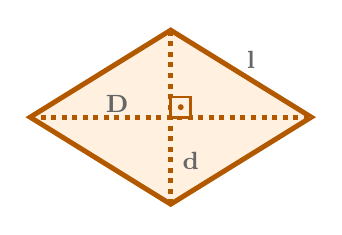
\begin{tikzpicture}[scale=0.85]
\draw[los] (0,1.3) -- (2.1,2.6) -- (4.2,1.3) -- (2.1,0) -- cycle;
\node[figno] at (2.4,0.65) {d};
\node[figno] at (1.3,1.5) {D};
\node[figno] at (3.3,2.15) {l};
\draw[los,dotted] (2.1,0) -- (2.1,2.6);
\draw[los,dotted] (0,1.3) -- (4.2,1.3);
\draw[los,figrect] (2.1,1.3) rectangle (2.4,1.6);
\filldraw[orange!70!black] (2.25,1.45) circle (1pt);
\end{tikzpicture}
\vspace{-4pt}\end{center}

\regra{$\displaystyle A = \frac{D \cdot d}{2} \qquad P = 4\,l$\\[6pt]
$\displaystyle l = \sqrt{\left(\frac{D}{2}\right)^{\!2}+\left(\frac{d}{2}\right)^{\!2}}$\\[2pt]
{\small $D$ = diagonal maior, $d$ = diagonal menor}}

\exemp{%
  Exemplo — $D=8,\; d=6$\\
  $l = \sqrt{4^2+3^2} = \sqrt{25} = \hlm{5}$\\[4pt]
  $A = \dfrac{8 \cdot 6}{2} = \hlm{24}$ \quad $P = 4 \cdot 5 = \hlm{20}$%
}

%─────────────────────────────────────────────────────────────
\TW{Circ}{badgegreen}{Círculo}{Área e comprimento da circunferência}

\begin{center}\vspace{-4pt}
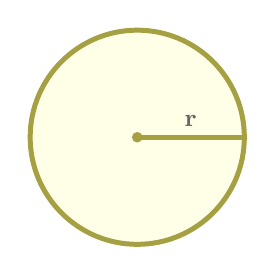
\begin{tikzpicture}[scale=0.85]
\draw[circ] (0,0) circle (1.6);
\filldraw[yellow!60!black] (0,0) circle (2pt);
\draw[circ] (0,0) -- (1.6,0);
\node[figno] at (0.8,0.25) {r};
\end{tikzpicture}
\vspace{-4pt}\end{center}

\regra{$A = \pi r^2 \qquad C = 2\pi r$\\[2pt]
{\small $r$ = raio, $C$ = circunferência, $\pi \approx 3{,}14159$}}

\exemp{%
  Exemplo — $r = 3$\\
  $A = \pi \cdot 9 = 9\pi \approx \hlm{28{,}27}$\\[4pt]
  $C = 6\pi \approx \hlm{18{,}85}$%
}

\nota{O \textbf{diâmetro} é $d = 2r$; pode-se escrever
$C = \pi d$ e $A = \pi\!\left(\dfrac{d}{2}\right)^{\!2}$.}

\end{multicols}

%─────────────────────────────────────────────────────────────
\vspace{6pt}
\TW{Tab}{badgegreen}{Resumo das Fórmulas}{Área (A) e Perímetro (P) de cada figura}

% Linha 1 — Quadrado · Retângulo · Paralelogramo
\vspace{6pt}\noindent
\begin{minipage}[t]{5.5cm}
\begin{tcolorbox}[arc=5pt, boxrule=0.8pt, colback=rulebg, colframe=darkblue,
  left=8pt, right=8pt, top=6pt, bottom=8pt]
{\color{darkblue}\bfseries\small QUADRADO}\par\vspace{4pt}
{\small\color{bodytext}$A = l^2$\par $P = 4\,l$}
\end{tcolorbox}
\end{minipage}\hfill
\begin{minipage}[t]{5.5cm}
\begin{tcolorbox}[arc=5pt, boxrule=0.8pt, colback=rulebg, colframe=darkblue,
  left=8pt, right=8pt, top=6pt, bottom=8pt]
{\color{darkblue}\bfseries\small RETÂNGULO}\par\vspace{4pt}
{\small\color{bodytext}$A = b \cdot h$\par $P = 2(b+h)$}
\end{tcolorbox}
\end{minipage}\hfill
\begin{minipage}[t]{5.5cm}
\begin{tcolorbox}[arc=5pt, boxrule=0.8pt, colback=rulebg, colframe=darkblue,
  left=8pt, right=8pt, top=6pt, bottom=8pt]
{\color{darkblue}\bfseries\small PARALELOGRAMO}\par\vspace{4pt}
{\small\color{bodytext}$A = b \cdot h$\par $P = 2(a+b)$}
\end{tcolorbox}
\end{minipage}

% Linha 2 — Triângulo · Equilátero · Trapézio
\vspace{6pt}\noindent
\begin{minipage}[t]{5.5cm}
\begin{tcolorbox}[arc=5pt, boxrule=0.8pt, colback=rulebg, colframe=darkblue,
  left=8pt, right=8pt, top=6pt, bottom=8pt]
{\color{darkblue}\bfseries\small TRIÂNGULO}\par\vspace{4pt}
{\small\color{bodytext}$A = \dfrac{b \cdot h}{2}$\par\vspace{3pt} $P = a+b+c$}
\end{tcolorbox}
\end{minipage}\hfill
\begin{minipage}[t]{5.5cm}
\begin{tcolorbox}[arc=5pt, boxrule=0.8pt, colback=rulebg, colframe=darkblue,
  left=8pt, right=8pt, top=6pt, bottom=8pt]
{\color{darkblue}\bfseries\small TRIÂNG. EQUILÁTERO}\par\vspace{4pt}
{\small\color{bodytext}$A = \dfrac{l^2\sqrt{3}}{4}$\par\vspace{3pt} $P = 3\,l$}
\end{tcolorbox}
\end{minipage}\hfill
\begin{minipage}[t]{5.5cm}
\begin{tcolorbox}[arc=5pt, boxrule=0.8pt, colback=rulebg, colframe=darkblue,
  left=8pt, right=8pt, top=6pt, bottom=8pt]
{\color{darkblue}\bfseries\small TRAPÉZIO}\par\vspace{4pt}
{\small\color{bodytext}$A = \dfrac{(B+b)\cdot h}{2}$\par\vspace{3pt} $P = a+b+c+d$}
\end{tcolorbox}
\end{minipage}

% Linha 3 — Losango · Círculo
\vspace{6pt}\noindent
\begin{minipage}[t]{8.7cm}
\begin{tcolorbox}[arc=5pt, boxrule=0.8pt, colback=rulebg, colframe=darkblue,
  left=8pt, right=8pt, top=6pt, bottom=8pt]
{\color{darkblue}\bfseries\small LOSANGO}\par\vspace{4pt}
{\small\color{bodytext}$A = \dfrac{D \cdot d}{2}$ \quad $P = 4\,l$\par\vspace{3pt}
$l = \sqrt{(D/2)^2+(d/2)^2}$}
\end{tcolorbox}
\end{minipage}\hfill
\begin{minipage}[t]{8.7cm}
\begin{tcolorbox}[arc=5pt, boxrule=0.8pt, colback=notebg, colframe=noteborder,
  left=8pt, right=8pt, top=6pt, bottom=8pt]
{\color{notetext}\bfseries\small CÍRCULO}\par\vspace{4pt}
{\small\color{bodytext}$A = \pi r^2$ \quad $C = 2\pi r$}
\end{tcolorbox}
\end{minipage}

\end{document}
